\documentclass{beamer}
\usepackage{amsmath}
\usepackage[english]{babel}
\usepackage{commath}
\usepackage[autostyle, english = american]{csquotes}
\usepackage{graphicx}
\usepackage{hyperref}
\usepackage{cleveref}
\usepackage[sort,round]{natbib}
\usepackage{parskip}
\usepackage{subcaption}

\usetheme{Boadilla}
\begin{document}
\title{Q-Learning on FPGA}
\author{Kevin Michael Frick \and Davide Ragazzini}
\institute{Università di Bologna}
\date{\today}
\setbeamercovered{transparent}
\begin{frame}
	\titlepage
\end{frame}

\begin{frame}
	\frametitle{Q-Learning}
	\begin{itemize}
		\item \emph{Off-policy}, \emph{classical} reinforcement learning algorithm
	\item Used to estimate an optimal policy in Markov decision processes, i.e. the policy that maximizes the expected value of the total reward over all successive steps
	\item The \emph{reward function} $Q(s, a)$ is approximated using a state-action matrix known as the Q-table
	\item After taking action $a$ in state $s$, obtaining reward $r$, $Q$ is updated following $Q'(s_t, a_t) \leftarrow Q(s_t, a_t) + \alpha (r_t + \gamma \max_a Q(s_{t+1}, a) - Q(s_t, a))$
	\item Falling $\alpha$ and $\epsilon$
	\end{itemize}
\end{frame}
\begin{frame}
	\frametitle{CartPole task}
	\begin{itemize}
		\item Learning a policy that can balance a pole on a rolling cart
		\item Physical system: inverted pendulum
		\item State space defined by $(x, \dot{x}, \theta, \dot{\theta})$
		\item Action space $A = \{x \leftarrow x + \delta x, x \leftarrow x - \delta x\}$.
	\end{itemize}
\end{frame}
\begin{frame}
	\frametitle{Vitis HLS}
	\begin{itemize}
		\item \texttt{learn()} as a top function, \texttt{update\_state()} and \texttt{discretize()} are factorized
		\item Space state mapped into 162 windows
		\item Port for status LEDs
		\item AXI Lite ports for return values, periods and Q-table
		\item AXI Stream port for the RNG
	\end{itemize}
\end{frame}

\begin{frame}
	\frametitle{Vivado}
	{

		\centering

		\includegraphics[width=\textwidth]{bd.png}

	}
\end{frame}
\begin{frame}
	\frametitle{Vitis}
	\begin{itemize}
		\item Initializes the Q-table over AXI Lite
		\item Sends the RNG seed over GPIO
		\item Automatically calculates average time to converge
	\end{itemize}
\end{frame}
\begin{frame}
	\frametitle{Experimental results}
	\begin{table}[h!]

\centering


\begin{tabular}{|l |l|}
  \hline & \textbf{Periods for convergence} \\ \hline
    \textbf{Random init in $[0, 1]$}             &  363                                                               \\ \hline
    \textbf{Random init in $[1, 2]$} &  329                                                               \\ \hline
    \textbf{Random init in $[2, 3]$} &  375                                                               \\ \hline
    \textbf{Random init in $[3, 4]$} &  426                                                               \\ \hline
    \textbf{Random init in $[4, 5]$} &  485                                                               \\ \hline
  \textbf{Init to 0}                 &  800                                                               \\ \hline
  \end{tabular}
  \caption{Average performance}
  \label{table:perf}
  \end{table}
\end{frame}
\begin{frame}
	\frametitle{Experimental results II}

	{

		\centering

		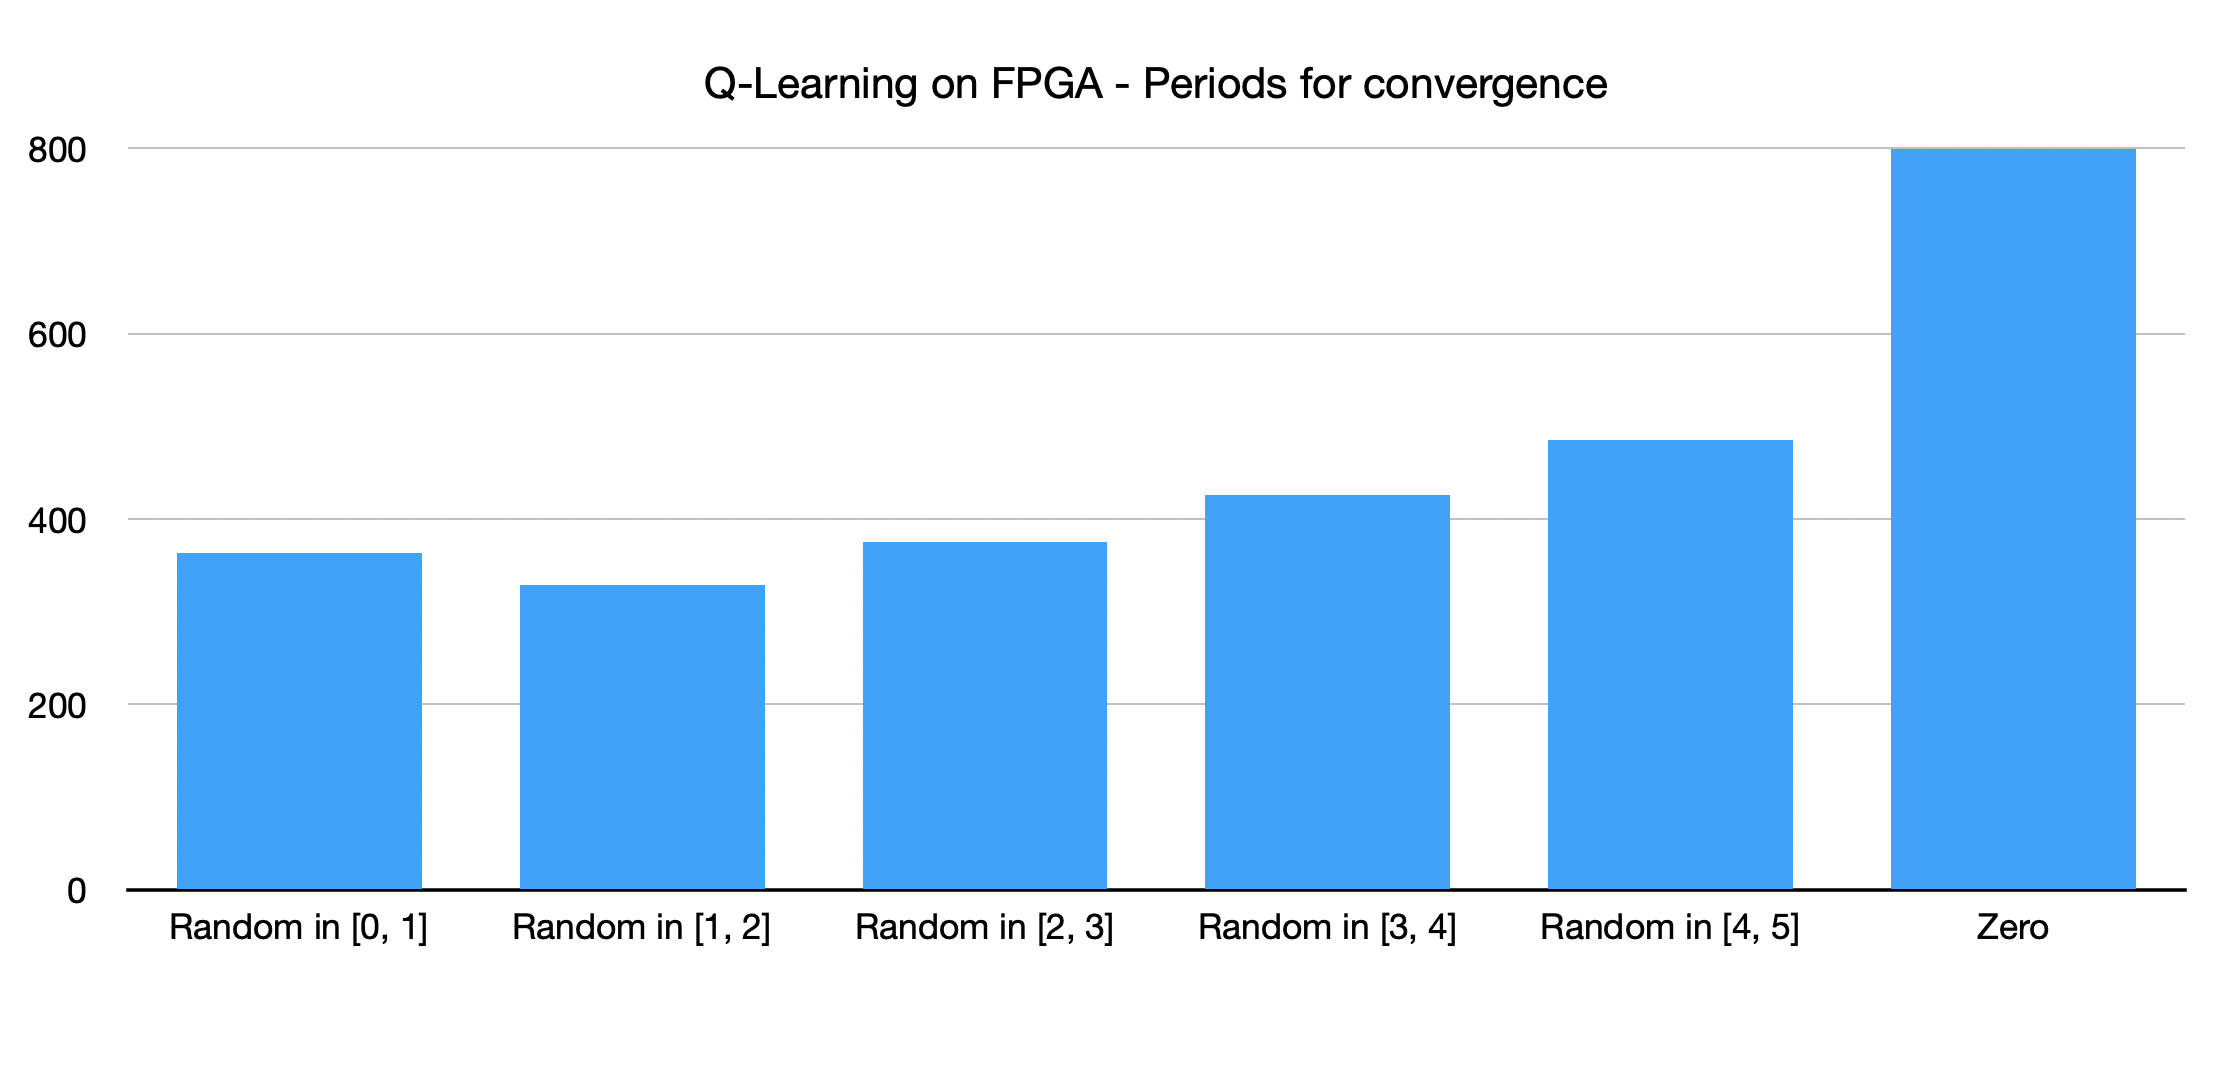
\includegraphics[width=\textwidth]{perf.png}

	}
\end{frame}
%\begin{frame}[allowframebreaks]
%	\frametitle{References}
%	\bibliographystyle{plainnat}
%	\nocite{*}
%	\bibliography{main}
%\end{frame}
\end{document}

